\icode{E-MD-CA-L2-261114-007}
如图所示，\(AC\)是半径为\(R\)的圆\(O\)的竖直直径，\(AB\)与\(AC\)的夹角为\(\theta\)，质量为\(m\)的小球（可视为质点）套在\(AB\)上，由\(B\)点静止释放，忽略一切摩擦，求小球滑到\(A\)点的时间。

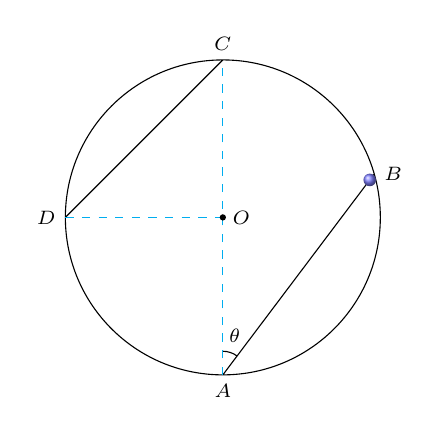
\begin{tikzpicture}[font=\scriptsize]
	\draw (0,2) circle(2) (0,0)node[below]{\(A\)}--(53:3.2)node[right]{\(B\)} (53:.3) arc(53:90:.3) (-2,2)--(0,4);
	\draw[dashed,cyan] (-2,2)--(0,2) (0,0)--(0,4);
	\node at(0,4)[above]{\(C\)} (0,2);
	\node at(-2,2)[left]{\(D\)};
	\shade[ball color=blue!50] (53:3.1) circle(.08);
	\fill (0,2)node[right]{\(O\)} circle(.04);
	\node at(.15,.5){\(\theta\)};
\end{tikzpicture}
\begin{answer}
    \(\sqrt{\frac{4R}{g}}\)
\end{answer}